%% bare_conf_compsoc.tex
%% V1.4b
%% 2015/08/26
%% by Michael Shell
%% See:
%% http://www.michaelshell.org/
%% for current contact information.
%%
%% This is a skeleton file demonstrating the use of IEEEtran.cls
%% (requires IEEEtran.cls version 1.8b or later) with an IEEE Computer
%% Society conference paper.
%%
%% Support sites:
%% http://www.michaelshell.org/tex/ieeetran/
%% http://www.ctan.org/pkg/ieeetran
%% and
%% http://www.ieee.org/

%%*************************************************************************
%% Legal Notice:
%% This code is offered as-is without any warranty either expressed or
%% implied; without even the implied warranty of MERCHANTABILITY or
%% FITNESS FOR A PARTICULAR PURPOSE! 
%% User assumes all risk.
%% In no event shall the IEEE or any contributor to this code be liable for
%% any damages or losses, including, but not limited to, incidental,
%% consequential, or any other damages, resulting from the use or misuse
%% of any information contained here.
%%
%% All comments are the opinions of their respective authors and are not
%% necessarily endorsed by the IEEE.
%%
%% This work is distributed under the LaTeX Project Public License (LPPL)
%% ( http://www.latex-project.org/ ) version 1.3, and may be freely used,
%% distributed and modified. A copy of the LPPL, version 1.3, is included
%% in the base LaTeX documentation of all distributions of LaTeX released
%% 2003/12/01 or later.
%% Retain all contribution notices and credits.
%% ** Modified files should be clearly indicated as such, including  **
%% ** renaming them and changing author support contact information. **
%%*************************************************************************


% *** Authors should verify (and, if needed, correct) their LaTeX system  ***
% *** with the testflow diagnostic prior to trusting their LaTeX platform ***
% *** with production work. The IEEE's font choices and paper sizes can   ***
% *** trigger bugs that do not appear when using other class files.       ***                          ***
% The testflow support page is at:
% http://www.michaelshell.org/tex/testflow/



\documentclass[conference,compsoc]{IEEEtran}
% Some/most Computer Society conferences require the compsoc mode option,
% but others may want the standard conference format.
%
% If IEEEtran.cls has not been installed into the LaTeX system files,
% manually specify the path to it like:
% \documentclass[conference,compsoc]{../sty/IEEEtran}


\usepackage{biblatex}
\usepackage[T1]{fontenc}
\usepackage{graphicx}
% Some very useful LaTeX packages include:
% (uncomment the ones you want to load)


% *** MISC UTILITY PACKAGES ***
%
%\usepackage{ifpdf}
% Heiko Oberdiek's ifpdf.sty is very useful if you need conditional
% compilation based on whether the output is pdf or dvi.
% usage:
% \ifpdf
%   % pdf code
% \else
%   % dvi code
% \fi
% The latest version of ifpdf.sty can be obtained from:
% http://www.ctan.org/pkg/ifpdf
% Also, note that IEEEtran.cls V1.7 and later provides a builtin
% \ifCLASSINFOpdf conditional that works the same way.
% When switching from latex to pdflatex and vice-versa, the compiler may
% have to be run twice to clear warning/error messages.






% *** CITATION PACKAGES ***
%
%\ifCLASSOPTIONcompsoc
  % IEEE Computer Society needs nocompress option
  % requires cite.sty v4.0 or later (November 2003)
 % \usepackage[nocompress]{cite}
%\else
  % normal IEEE
 % \usepackage{cite}
%\fi
% cite.sty was written by Donald Arseneau
% V1.6 and later of IEEEtran pre-defines the format of the cite.sty package
% \cite{} output to follow that of the IEEE. Loading the cite package will
% result in citation numbers being automatically sorted and properly
% "compressed/ranged". e.g., [1], [9], [2], [7], [5], [6] without using
% cite.sty will become [1], [2], [5]--[7], [9] using cite.sty. cite.sty's
% \cite will automatically add leading space, if needed. Use cite.sty's
% noadjust option (cite.sty V3.8 and later) if you want to turn this off
% such as if a citation ever needs to be enclosed in parenthesis.
% cite.sty is already installed on most LaTeX systems. Be sure and use
% version 5.0 (2009-03-20) and later if using hyperref.sty.
% The latest version can be obtained at:
% http://www.ctan.org/pkg/cite
% The documentation is contained in the cite.sty file itself.
%
% Note that some packages require special options to format as the Computer
% Society requires. In particular, Computer Society  papers do not use
% compressed citation ranges as is done in typical IEEE papers
% (e.g., [1]-[4]). Instead, they list every citation separately in order
% (e.g., [1], [2], [3], [4]). To get the latter we need to load the cite
% package with the nocompress option which is supported by cite.sty v4.0
% and later.





% *** GRAPHICS RELATED PACKAGES ***
%
\ifCLASSINFOpdf
  % \usepackage[pdftex]{graphicx}
  % declare the path(s) where your graphic files are
  % \graphicspath{{../pdf/}{../jpeg/}}
  % and their extensions so you won't have to specify these with
  % every instance of \includegraphics
  % \DeclareGraphicsExtensions{.pdf,.jpeg,.png}
\else
  % or other class option (dvipsone, dvipdf, if not using dvips). graphicx
  % will default to the driver specified in the system graphics.cfg if no
  % driver is specified.
  % \usepackage[dvips]{graphicx}
  % declare the path(s) where your graphic files are
  % \graphicspath{{../eps/}}
  % and their extensions so you won't have to specify these with
  % every instance of \includegraphics
  % \DeclareGraphicsExtensions{.eps}
\fi
% graphicx was written by David Carlisle and Sebastian Rahtz. It is
% required if you want graphics, photos, etc. graphicx.sty is already
% installed on most LaTeX systems. The latest version and documentation
% can be obtained at: 
% http://www.ctan.org/pkg/graphicx
% Another good source of documentation is "Using Imported Graphics in
% LaTeX2e" by Keith Reckdahl which can be found at:
% http://www.ctan.org/pkg/epslatex
%
% latex, and pdflatex in dvi mode, support graphics in encapsulated
% postscript (.eps) format. pdflatex in pdf mode supports graphics
% in .pdf, .jpeg, .png and .mps (metapost) formats. Users should ensure
% that all non-photo figures use a vector format (.eps, .pdf, .mps) and
% not a bitmapped formats (.jpeg, .png). The IEEE frowns on bitmapped formats
% which can result in "jaggedy"/blurry rendering of lines and letters as
% well as large increases in file sizes.
%
% You can find documentation about the pdfTeX application at:
% http://www.tug.org/applications/pdftex





% *** MATH PACKAGES ***
%
%\usepackage{amsmath}
% A popular package from the American Mathematical Society that provides
% many useful and powerful commands for dealing with mathematics.
%
% Note that the amsmath package sets \interdisplaylinepenalty to 10000
% thus preventing page breaks from occurring within multiline equations. Use:
%\interdisplaylinepenalty=2500
% after loading amsmath to restore such page breaks as IEEEtran.cls normally
% does. amsmath.sty is already installed on most LaTeX systems. The latest
% version and documentation can be obtained at:
% http://www.ctan.org/pkg/amsmath





% *** SPECIALIZED LIST PACKAGES ***
%
%\usepackage{algorithmic}
% algorithmic.sty was written by Peter Williams and Rogerio Brito.
% This package provides an algorithmic environment fo describing algorithms.
% You can use the algorithmic environment in-text or within a figure
% environment to provide for a floating algorithm. Do NOT use the algorithm
% floating environment provided by algorithm.sty (by the same authors) or
% algorithm2e.sty (by Christophe Fiorio) as the IEEE does not use dedicated
% algorithm float types and packages that provide these will not provide
% correct IEEE style captions. The latest version and documentation of
% algorithmic.sty can be obtained at:
% http://www.ctan.org/pkg/algorithms
% Also of interest may be the (relatively newer and more customizable)
% algorithmicx.sty package by Szasz Janos:
% http://www.ctan.org/pkg/algorithmicx




% *** ALIGNMENT PACKAGES ***
%
%\usepackage{array}
% Frank Mittelbach's and David Carlisle's array.sty patches and improves
% the standard LaTeX2e array and tabular environments to provide better
% appearance and additional user controls. As the default LaTeX2e table
% generation code is lacking to the point of almost being broken with
% respect to the quality of the end results, all users are strongly
% advised to use an enhanced (at the very least that provided by array.sty)
% set of table tools. array.sty is already installed on most systems. The
% latest version and documentation can be obtained at:
% http://www.ctan.org/pkg/array


% IEEEtran contains the IEEEeqnarray family of commands that can be used to
% generate multiline equations as well as matrices, tables, etc., of high
% quality.




% *** SUBFIGURE PACKAGES ***
%\ifCLASSOPTIONcompsoc
%  \usepackage[caption=false,font=footnotesize,labelfont=sf,textfont=sf]{subfig}
%\else
%  \usepackage[caption=false,font=footnotesize]{subfig}
%\fi
% subfig.sty, written by Steven Douglas Cochran, is the modern replacement
% for subfigure.sty, the latter of which is no longer maintained and is
% incompatible with some LaTeX packages including fixltx2e. However,
% subfig.sty requires and automatically loads Axel Sommerfeldt's caption.sty
% which will override IEEEtran.cls' handling of captions and this will result
% in non-IEEE style figure/table captions. To prevent this problem, be sure
% and invoke subfig.sty's "caption=false" package option (available since
% subfig.sty version 1.3, 2005/06/28) as this is will preserve IEEEtran.cls
% handling of captions.
% Note that the Computer Society format requires a sans serif font rather
% than the serif font used in traditional IEEE formatting and thus the need
% to invoke different subfig.sty package options depending on whether
% compsoc mode has been enabled.
%
% The latest version and documentation of subfig.sty can be obtained at:
% http://www.ctan.org/pkg/subfig



% *** FLOAT PACKAGES ***
%
%\usepackage{fixltx2e}
% fixltx2e, the successor to the earlier fix2col.sty, was written by
% Frank Mittelbach and David Carlisle. This package corrects a few problems
% in the LaTeX2e kernel, the most notable of which is that in current
% LaTeX2e releases, the ordering of single and double column floats is not
% guaranteed to be preserved. Thus, an unpatched LaTeX2e can allow a
% single column figure to be placed prior to an earlier double column
% figure.
% Be aware that LaTeX2e kernels dated 2015 and later have fixltx2e.sty's
% corrections already built into the system in which case a warning will
% be issued if an attempt is made to load fixltx2e.sty as it is no longer
% needed.
% The latest version and documentation can be found at:
% http://www.ctan.org/pkg/fixltx2e


%\usepackage{stfloats}
% stfloats.sty was written by Sigitas Tolusis. This package gives LaTeX2e
% the ability to do double column floats at the bottom of the page as well
% as the top. (e.g., "\begin{figure*}[!b]" is not normally possible in
% LaTeX2e). It also provides a command:
%\fnbelowfloat
% to enable the placement of footnotes below bottom floats (the standard
% LaTeX2e kernel puts them above bottom floats). This is an invasive package
% which rewrites many portions of the LaTeX2e float routines. It may not work
% with other packages that modify the LaTeX2e float routines. The latest
% version and documentation can be obtained at:
% http://www.ctan.org/pkg/stfloats
% Do not use the stfloats baselinefloat ability as the IEEE does not allow
% \baselineskip to stretch. Authors submitting work to the IEEE should note
% that the IEEE rarely uses double column equations and that authors should try
% to avoid such use. Do not be tempted to use the cuted.sty or midfloat.sty
% packages (also by Sigitas Tolusis) as the IEEE does not format its papers in
% such ways.
% Do not attempt to use stfloats with fixltx2e as they are incompatible.
% Instead, use Morten Hogholm'a dblfloatfix which combines the features
% of both fixltx2e and stfloats:
%
% \usepackage{dblfloatfix}
% The latest version can be found at:
% http://www.ctan.org/pkg/dblfloatfix


\usepackage{amsmath}

% *** PDF, URL AND HYPERLINK PACKAGES ***
%
%\usepackage{url}
% url.sty was written by Donald Arseneau. It provides better support for
% handling and breaking URLs. url.sty is already installed on most LaTeX
% systems. The latest version and documentation can be obtained at:
% http://www.ctan.org/pkg/url
% Basically, \url{my_url_here}.




% *** Do not adjust lengths that control margins, column widths, etc. ***
% *** Do not use packages that alter fonts (such as pslatex).         ***
% There should be no need to do such things with IEEEtran.cls V1.6 and later.
% (Unless specifically asked to do so by the journal or conference you plan
% to submit to, of course. )


% correct bad hyphenation here
\hyphenation{op-tical net-works semi-conduc-tor}

\addbibresource{references.bib}

\begin{document}
%
% paper title
% Titles are generally capitalized except for words such as a, an, and, as,
% at, but, by, for, in, nor, of, on, or, the, to and up, which are usually
% not capitalized unless they are the first or last word of the title.
% Linebreaks \\ can be used within to get better formatting as desired.
% Do not put math or special symbols in the title.
\title{Symbolic music generation using Mamba architecture}


% author names and affiliations
% use a multiple column layout for up to three different
% affiliations
%\author{\IEEEauthorblockN{Michael Shell}
%\IEEEauthorblockA{School of Electrical and\\Computer Engineering\\
%Georgia Institute of Technology\\
%Atlanta, Georgia 30332--0250\\
%Email: http://www.michaelshell.org/contact.html}
%\and
%\IEEEauthorblockN{Homer Simpson}
%\IEEEauthorblockA{Twentieth Century Fox\\
%Springfield, USA\\
%Email: homer@thesimpsons.com}
%\and
%\IEEEauthorblockN{James Kirk\\ and Montgomery Scott}
%\IEEEauthorblockA{Starfleet Academy\\
%San Francisco, California 96678-2391\\
%Telephone: (800) 555--1212\\
%Fax: (888) 555--1212}}
\author{\IEEEauthorblockN{Jan Retkowski} \and \IEEEauthorblockN{Miłosz Łopatto}
    \IEEEauthorblockA{\textit{Faculty of Electronics and Information Technology} \\
        \textit{Warsaw University of Technology}\\
        Warszawa, Polska \\
        TODO: emails}
    \and \IEEEauthorblockN{Jakub Stępniak}}

% conference papers do not typically use \thanks and this command
% is locked out in conference mode. If really needed, such as for
% the acknowledgment of grants, issue a \IEEEoverridecommandlockouts
% after \documentclass

% for over three affiliations, or if they all won't fit within the width
% of the page (and note that there is less available width in this regard for
% compsoc conferences compared to traditional conferences), use this
% alternative format:
% 
%\author{\IEEEauthorblockN{Michael Shell\IEEEauthorrefmark{1},
%Homer Simpson\IEEEauthorrefmark{2},
%James Kirk\IEEEauthorrefmark{3}, 
%Montgomery Scott\IEEEauthorrefmark{3} and
%Eldon Tyrell\IEEEauthorrefmark{4}}
%\IEEEauthorblockA{\IEEEauthorrefmark{1}School of Electrical and Computer Engineering\\
%Georgia Institute of Technology,
%Atlanta, Georgia 30332--0250\\ Email: see http://www.michaelshell.org/contact.html}
%\IEEEauthorblockA{\IEEEauthorrefmark{2}Twentieth Century Fox, Springfield, USA\\
%Email: homer@thesimpsons.com}
%\IEEEauthorblockA{\IEEEauthorrefmark{3}Starfleet Academy, San Francisco, California 96678-2391\\
%Telephone: (800) 555--1212, Fax: (888) 555--1212}
%\IEEEauthorblockA{\IEEEauthorrefmark{4}Tyrell Inc., 123 Replicant Street, Los Angeles, California 90210--4321}}




% use for special paper notices
%\IEEEspecialpapernotice{(Invited Paper)}




% make the title area
\maketitle

% As a general rule, do not put math, special symbols or citations
% in the abstract
\begin{abstract}
    Over the past few years, a lot of effort has been put into making Transformers more and more efficient. However, they still suffer from quadratic memory and inference time complexity.  Recently they have been experiencing increasing competition from state space models (SSMs), that avoid some of transformer's drawbacks. In this paper we test one of state of the art SSM models called Mamba in symbolic music generation. To achieve this we conducted several experiments on MAESTRO MIDI dataset. Our results show that TODO
\end{abstract}

% no keywords

\begin{IEEEkeywords}
    deep leraning, transformer, music, symbolic music generation, neural network, generative, unsupervised learning, state space model, ssm, mamba
\end{IEEEkeywords}


% For peer review papers, you can put extra information on the cover
% page as needed:
% \ifCLASSOPTIONpeerreview
% \begin{center} \bfseries EDICS Category: 3-BBND \end{center}
% \fi
%
% For peerreview papers, this IEEEtran command inserts a page break and
% creates the second title. It will be ignored for other modes.
\IEEEpeerreviewmaketitle



\section{Introduction}
% no \IEEEPARstart
Symbolic music generation has been an area of active research over the past decades. In the beginning it was dominated by classical methods like Hidden Markov Models. During the advent of deep learning in the last decade, neural networks managed to become a go to method for this task. During those years a lot of architectures, including Long Short-term Memory networks (LSTMs) \cite{lstm}, Variational Autoencoders (VAEs) \cite{kingma2022autoencoding} and Generative Adversarial Networks (GANs) \cite{goodfellow2014generative} were used to successfully generate music in symbolic formats. However, after popularisation of Transformers \cite{attention-is-all-you-need} and Diffusion Models \cite{ho2020denoising} in the field broad of deep learning, they seem to be gaining more and more dominance in the area of symbolic music generation.  In the case of transformers, which are the go to architecture in the area of natural language processing, a lot of effort has been put into small iterative improvements, to make the more efficient. However, they still suffer from quadratic GPU memory, as well as inference time complexity. To mitigate those problems State Space Models (SSMs) \cite{ssm} were developed.  Recently they have been experiencing gaining popularity and even beating transformers on some of their most signature tasks in the field of nature language processing, while being significantly smaller \cite{mamba}. They seem to be especially suited for long time dependencies. Musical data, which often contains such long dependencies seem to be suited to further test the performance of SSMs. Therefore we decided to use current state of the art SSM model called Mamba \cite{mamba} to generate music in symbolic format.


%\hfill mds

%\hfill August 26, 2015

%\subsection{Subsection Heading Here}
%Subsection text here.


%\subsubsection{Subsubsection Heading Here}
%Subsubsection text here.


%\clearpage
\section{Data}
We decided to use MIDI \cite{midi} music representation. It is by far the most popular format in the field of symbolic music and allows us to freely use the largest symbolic music datasets available. Because of model's size a lot of data is required to reduce the chance of overfitting. The dataset we chose is MAESTRO (MIDI and Audio Edited for Synchronous TRacks and Organization) \cite{maestro1} \cite{maestro2} . It contains over 200 hours of virtuosic piano performances. The data comes from ten years of International Piano-e-Competition. It is one of the most popular datasets, which allows us to easily compare our results to other models. The data was downloaded using Muspy \cite{muspy} library, which allows for convenient handling of symbolic musical data. The tokenization was conducted using miditok \cite{miditok2021} library. It contains methods for tokenising MIDI data into most of the most popular formats. We decided to opt for REMI \cite{remi} format with learned Byte-Pair Encodings.

\section{Architecture}
Mamba utilises a novel approach called selective state space models (SSMs), which enhance traditional state space models by allowing
parameters to be functions of the input. This design enables the model to selectively propagate or forget information along the sequence length,
dependent on the current input token. Mamba integrates this selective SSM approach into a simplified end-to-end architecture, foregoing traditional components
like attention or MLP blocks found in architectures like Transformers.

The main difference between Selective SSM and traditional SSM is the input-dependence, which mimics what the attention mechanism in Transformers
does—essentially assessing whether a specific token is important or not. However, this feature sacrifices the ability of traditional SSMs
to precompute all learnable matrices ($\Delta$, A, B, C) and their configurations based on sequence length in a single inference pass.
To address this, we introduce a mechanism of Parallel Associative Scan (similar to Prefix Sum) that requires storing precomputed calculations,
leading to higher memory usage but still maintaining linear computation.

\begin{figure}[!htbp]
    \centering 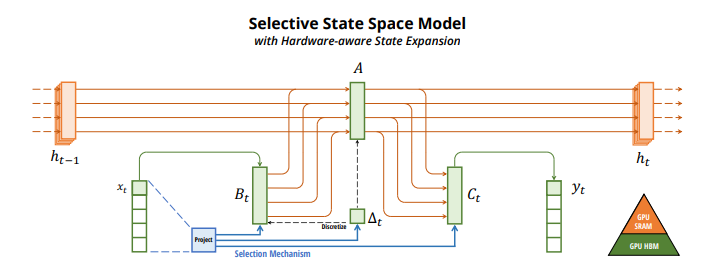
\includegraphics[width=\linewidth]{../assets/SelectiveSSM.png}
    \caption{Selective SSM \cite{mamba}}
    \label{fig:ssm}
\end{figure}

To enhance efficiency further, the authors proposed using a hardware-aware algorithm that leverages two main types of GPU memory:
SRAM, which is fast but has limited capacity (ideal for matrix calculations), and HBM, which is slower but has a larger capacity.
The main bottleneck of this approach is managing the data transfer between these memory types.

\begin{figure}[!htbp]
    \centering 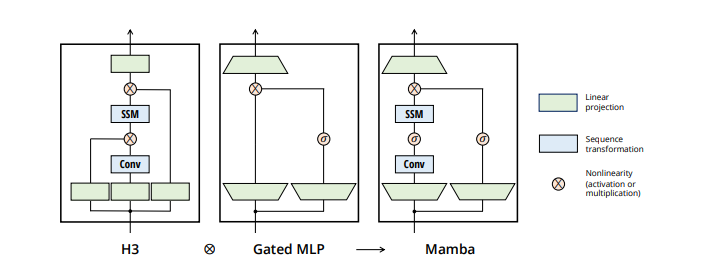
\includegraphics[width=\linewidth]{../assets/Mamba.png}
    \caption{Mamba block \cite{mamba}}
    \label{fig:mamba}
\end{figure}

Selective SSM is a crucial component of the Mamba block, but the system also includes linear layers that increase dimensionality, nonlinear layers, and gating connections.
Whole architecture is build from many Mamba block which are computed layer by layer.


\begin{table}[t] \centering
    % Podpis tabeli umieszczamy od góry
    \caption{Model comparison \cite{mamba}}
    \label{tab:comparison}

    % Tabela z trzema kolumnami:
    % dwie wyrównanie do środka [c], a ostatnia do prawej [r]
    % szerokość kolumn automatyczna (równa szerokości tekstu)
    \resizebox{\linewidth}{!}{\begin{tabular}{| c | c | c | c |} \hline
            Architecture          & Complexity & Memory   & Performance \\ \hline\hline
            Transformer           & $ O(N^2)$  & $O(N^2)$ & great       \\ \hline
            RNN                   & $O(N)$     & $O(N)$   & poor        \\ \hline
            SSM                   & $O(N)$     & $O(N)$   & poor        \\ \hline
            Selective SSM (Mamba) & $O(N)$     & $O(N)$   & great.      \\ \hline
            % Komórka o szerokości dwóch kolumn, wyrównana do prawej
            % Przypisy dolne w tabelach wstawiamy przez \tablefootnote
            % \multicolumn{2}{|r|}{Suma\tablefootnote{Table footnote.}} & 123,45 \\ \hline
        \end{tabular}}
\end{table}

\begin{figure}[!htbp]
    \centering 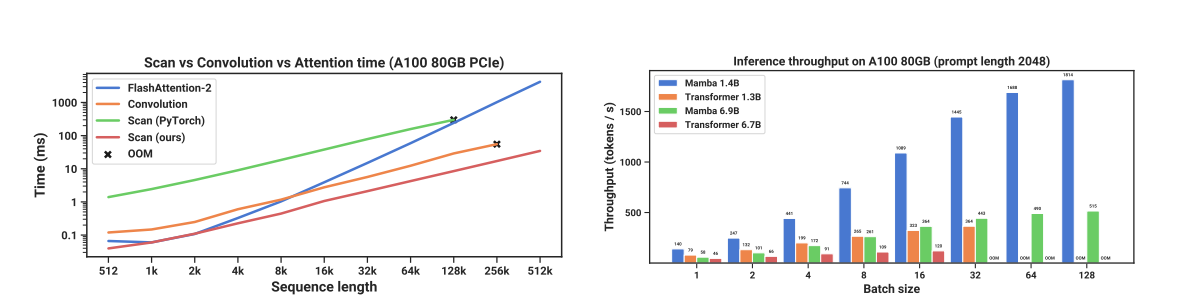
\includegraphics[width=\linewidth]{../assets/results.png}
    \caption{Benchmarks \cite{mamba}}
    \label{fig:mamba}
\end{figure}

\section{Training Setup}
TODO
\section{Experiments}
\subsection{Synthetic Data}
To first check that our training setup is correct we decided to overfit the model to synthetic data. For this purpose we generated sequence $0, 1, ..., 1999$ the tried to make model recreate it after receiving 0 token as input. During the training loss quickly approached zero. When testing the model it managed to generate the entire sequence correctly, abeit it required tuning the generation function's parameters.

\begin{figure}[!htbp]
    \centering 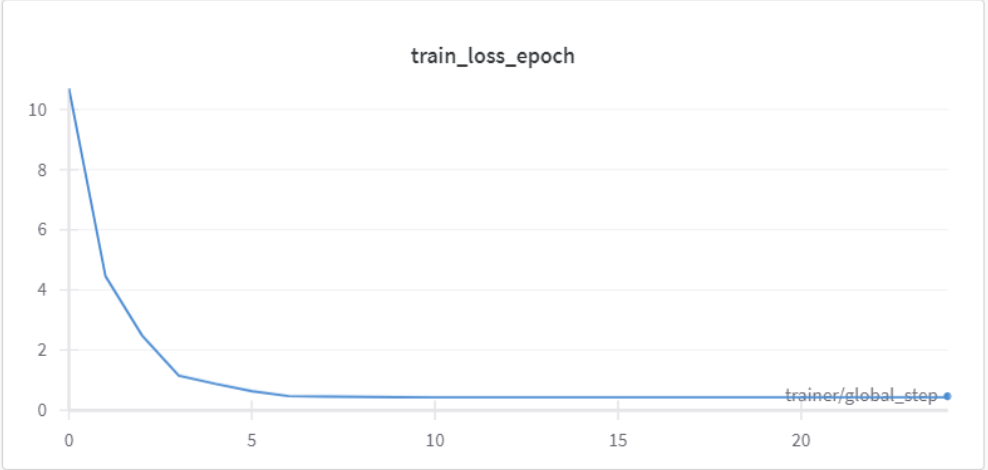
\includegraphics[width=\linewidth]{../assets/synth_data_train.png}
    \caption{ Loss during training on synthetic data}
    \label{fig:synth}
\end{figure}

TODO: second version:
We conducted a series of experiments to evaluate the performance of the Mamba architecture in symbolic music generation. The experiments are outlined as follows:

\begin{enumerate}
    \item \textbf{Simple Sequence Training}: We began by training the model on a simple numerical sequence (e.g., 0, 1, 2, 3, 4, ...). This experiment was designed to verify the model's ability to learn and reproduce basic patterns. The main goal of this part was to catch any implementation bugs as soon as possible.

    \item \textbf{Single Musical Piece Training}: Next, we trained the model on a single musical piece. This experiment aimed to assess the model's capacity to understand and generate music from a limited dataset. Even though it may seem to be a trivial task, playing with configuration was necessary – both training and inference.

    \item \textbf{Comprehensive Training on Multiple Pieces}: Finally, we conducted full-scale training using a diverse set of musical pieces from the MAESTRO dataset. This experiment was intended to evaluate the model's performance in generating complex and varied musical compositions.
\end{enumerate}

Each experiment was carefully monitored, and the generated outputs were analyzed to determine the model's effectiveness in capturing musical structures and patterns.

\begin{figure}[!htbp]
    \centering 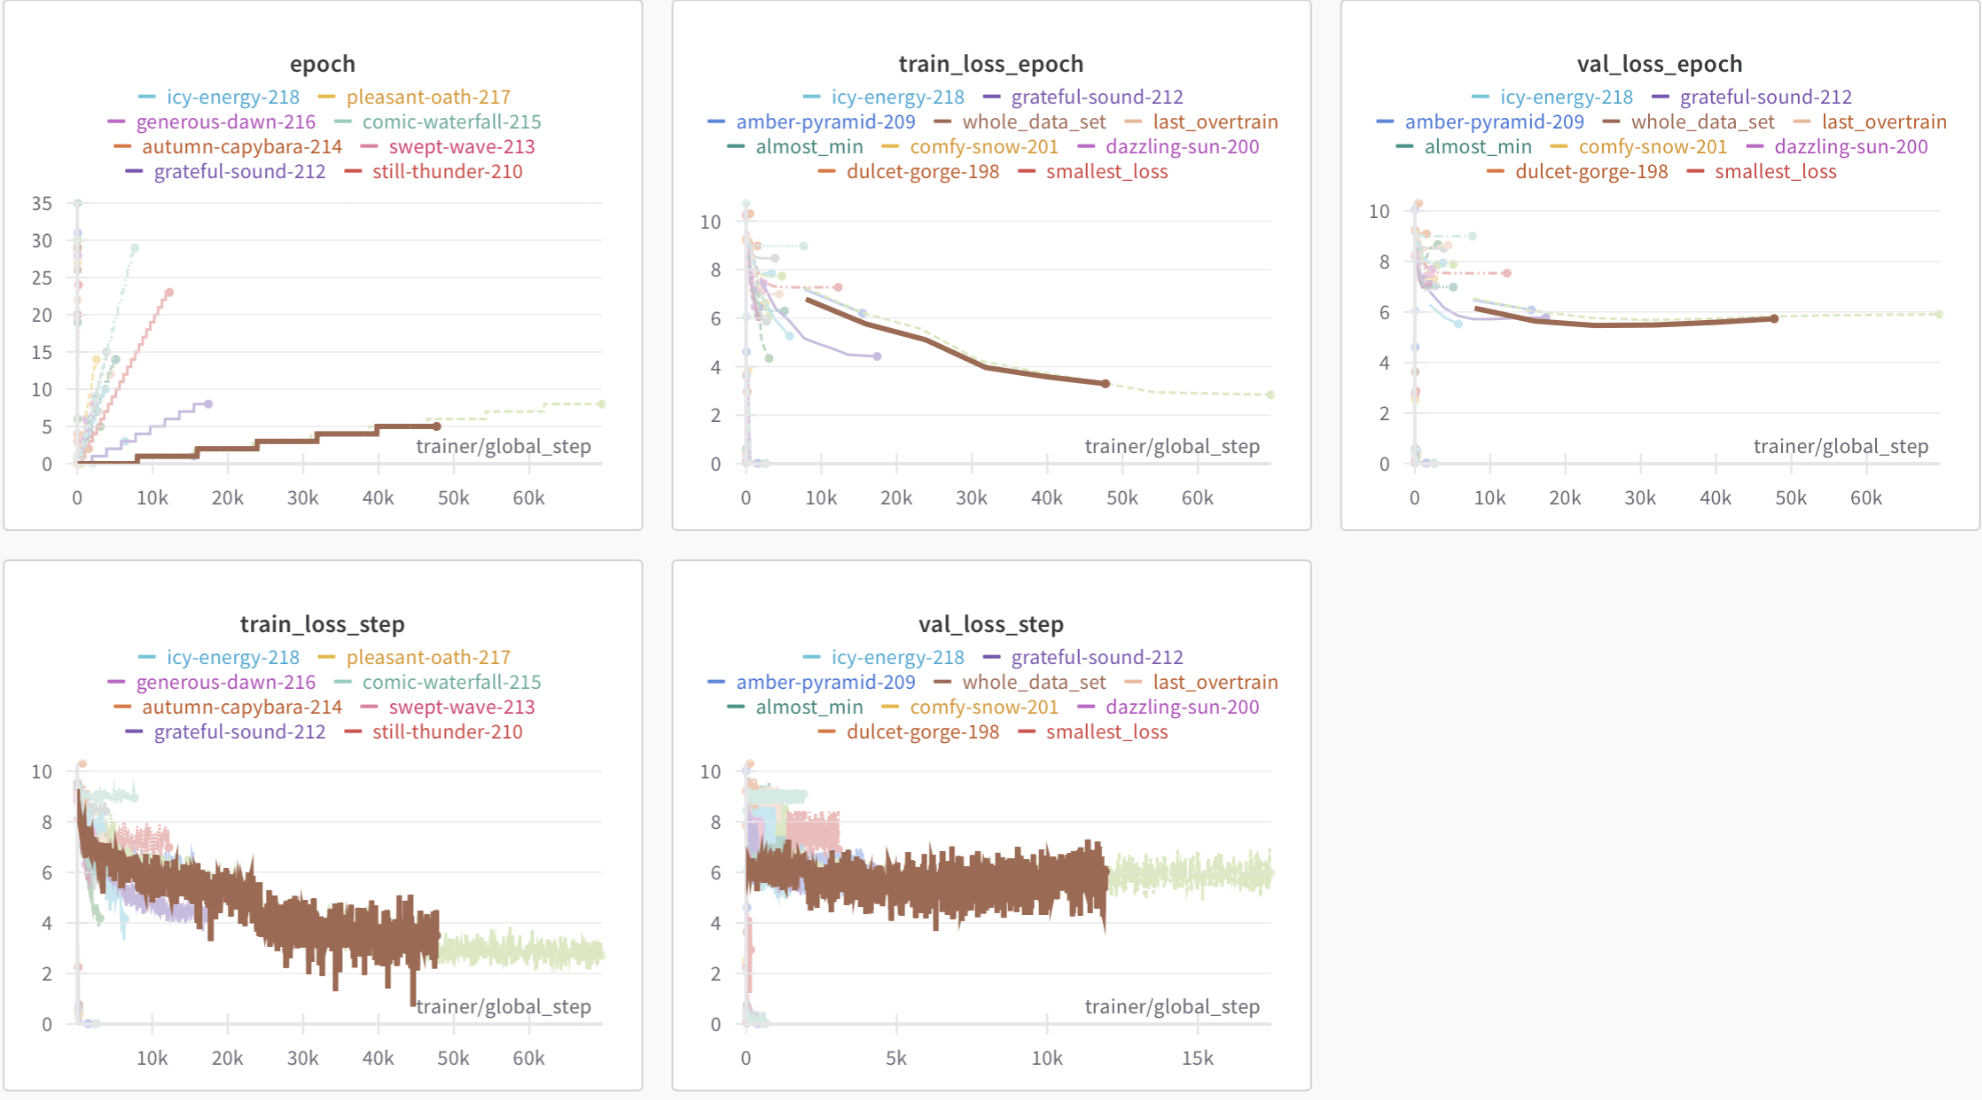
\includegraphics[width=\linewidth]{../assets/train.png}
    \caption{Training and validation losses in various experiments}
    \label{fig:synth}
\end{figure}

\section{Conclusions}
Although mamba managed to generate novel samples, they weren't of high quality. This may be due our models being unable to handle the complexities of virtuosic music. The model might be more suited for simpler datasets that do not contain such intricate musical scores. 

\subsection{Future work}
While Mamba offers better performance than transformers, it comes at the cost of output quality. A promising direction for future research is to experiment with hybrid architectures that combine the strengths of both models. Examples of such architectures include \textbf{MambaFormer} \cite{mambaformer} and \textbf{Jamba} \cite{jamba}. It is also worth trying different datasets, to see how mamba handles them.

% An example of a floating figure using the graphicx package.
% Note that \label must occur AFTER (or within) \caption.
% For figures, \caption should occur after the \includegraphics.
% Note that IEEEtran v1.7 and later has special internal code that
% is designed to preserve the operation of \label within \caption
% even when the captionsoff option is in effect. However, because
% of issues like this, it may be the safest practice to put all your
% \label just after \caption rather than within \caption{}.
%
% Reminder: the "draftcls" or "draftclsnofoot", not "draft", class
% option should be used if it is desired that the figures are to be
% displayed while in draft mode.
%
%\begin{figure}[!t]
%\centering
%\includegraphics[width=2.5in]{myfigure}
% where an .eps filename suffix will be assumed under latex, 
% and a .pdf suffix will be assumed for pdflatex; or what has been declared
% via \DeclareGraphicsExtensions.
%\caption{Simulation results for the network.}
%\label{fig_sim}
%\end{figure}

% Note that the IEEE typically puts floats only at the top, even when this
% results in a large percentage of a column being occupied by floats.


% An example of a double column floating figure using two subfigures.
% (The subfig.sty package must be loaded for this to work.)
% The subfigure \label commands are set within each subfloat command,
% and the \label for the overall figure must come after \caption.
% \hfil is used as a separator to get equal spacing.
% Watch out that the combined width of all the subfigures on a 
% line do not exceed the text width or a line break will occur.
%
%\begin{figure*}[!t]
%\centering
%\subfloat[Case I]{\includegraphics[width=2.5in]{box}%
%\label{fig_first_case}}
%\hfil
%\subfloat[Case II]{\includegraphics[width=2.5in]{box}%
%\label{fig_second_case}}
%\caption{Simulation results for the network.}
%\label{fig_sim}
%\end{figure*}
%
% Note that often IEEE papers with subfigures do not employ subfigure
% captions (using the optional argument to \subfloat[]), but instead will
% reference/describe all of them (a), (b), etc., within the main caption.
% Be aware that for subfig.sty to generate the (a), (b), etc., subfigure
% labels, the optional argument to \subfloat must be present. If a
% subcaption is not desired, just leave its contents blank,
% e.g., \subfloat[].


% An example of a floating table. Note that, for IEEE style tables, the
% \caption command should come BEFORE the table and, given that table
% captions serve much like titles, are usually capitalized except for words
% such as a, an, and, as, at, but, by, for, in, nor, of, on, or, the, to
% and up, which are usually not capitalized unless they are the first or
% last word of the caption. Table text will default to \footnotesize as
% the IEEE normally uses this smaller font for tables.
% The \label must come after \caption as always.
%
%\begin{table}[!t]
%% increase table row spacing, adjust to taste
%\renewcommand{\arraystretch}{1.3}
% if using array.sty, it might be a good idea to tweak the value of
% \extrarowheight as needed to properly center the text within the cells
%\caption{An Example of a Table}
%\label{table_example}
%\centering
%% Some packages, such as MDW tools, offer better commands for making tables
%% than the plain LaTeX2e tabular which is used here.
%\begin{tabular}{|c||c|}
%\hline
%One & Two\\
%\hline
%Three & Four\\
%\hline
%\end{tabular}
%\end{table}


% Note that the IEEE does not put floats in the very first column
% - or typically anywhere on the first page for that matter. Also,
% in-text middle ("here") positioning is typically not used, but it
% is allowed and encouraged for Computer Society conferences (but
% not Computer Society journals). Most IEEE journals/conferences use
% top floats exclusively. 
% Note that, LaTeX2e, unlike IEEE journals/conferences, places
% footnotes above bottom floats. This can be corrected via the
% \fnbelowfloat command of the stfloats package.


% conference papers do not normally have an appendix



% use section* for acknowledgment
%\ifCLASSOPTIONcompsoc
% The Computer Society usually uses the plural form
%\section*{Acknowledgments}
%\else
% regular IEEE prefers the singular form
%  \section*{Acknowledgment}
%\fi


%The authors would like to thank...





% trigger a \newpage just before the given reference
% number - used to balance the columns on the last page
% adjust value as needed - may need to be readjusted if
% the document is modified later
%\IEEEtriggeratref{8}
% The "triggered" command can be changed if desired:
%\IEEEtriggercmd{\enlargethispage{-5in}}

% references section

% can use a bibliography generated by BibTeX as a .bbl file
% BibTeX documentation can be easily obtained at:
% http://mirror.ctan.org/biblio/bibtex/contrib/doc/
% The IEEEtran BibTeX style support page is at:
% http://www.michaelshell.org/tex/ieeetran/bibtex/
%\bibliographystyle{IEEEtran}
% argument is your BibTeX string definitions and bibliography database(s)
%\bibliography{IEEEabrv,../bib/paper}
%\bibliography{artykul}
%
% <OR> manually copy in the resultant .bbl file
% set second argument of \begin to the number of references
% (used to reserve space for the reference number labels box)
%\begin{thebibliography}{1}

%\bibitem{IEEEhowto:kopka}
%H.~Kopka and P.~W. Daly, \emph{A Guide to \LaTeX}, 3rd~ed.\hskip 1em plus
% 0.5em minus 0.4em\relax Harlow, England: Addison-Wesley, 1999.

%\end{thebibliography}

\printbibliography


% that's all folks
\end{document}